\textbf{6.1.} 长度 $10\mathrm{cm}$ 的导线置于均匀磁场中， $B = (2e_x - 3e_y + 5e_z)\mathrm{T}$ . 此线载有电流3A，流动方向与 $-e_x + 4e_y + 3e_z$ 平行，求磁场作用于导线上的总力 $\pmb{F}$ .

\vfill

\textbf{6.2.} 惠斯登电桥由边长为 $a$ 的正方形构成(习题6.2图)，它被放在磁场 $\pmb{B}$ 中， $\pmb{B}$ 平行于电桥所在的平面并与包含检流计的支路平行，流入电桥的总电流是 $I$ 。

（1）作用在电桥上的净力 $\pmb{F}$ 是多少？

（2）此解答是否依赖于电桥平衡？

\begin{center}
    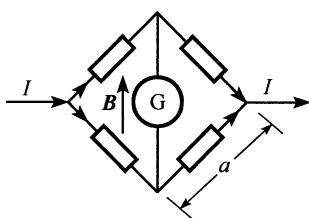
\includegraphics[width=0.3\linewidth]{figures/fig_6_3.jpg}
\end{center}

\vfill

\newpage

\textbf{6.3.} 一个半径为 $R$ 、载有电流 $I$ 的圆形回路处于一恒定磁场 $\pmb{B}$ 中， $\pmb{B}$ 垂直于回路平面，与电流满足右手螺旋关系。

(1) 求圆导线内部的张力；

(2) 若 $I=7.0A, R=5.0\times10^{-2}m, B=1.0Wb\cdot m^{-2}$ ，计算张力大小.


\vfill

\textbf{6.4.} 一段导线弯成习题 6.4 图所示的形状, 它的质量为 $m$ . 上面水平一段长为 $l$ , 处在均匀磁场中, 磁感应强度 $\pmb{B}$ 与导线垂直. 导线下面两端分别插在两个浅水银槽里, 并通过水银槽与一带开关 $\mathbf{K}$ 的外电源连接. 当 $\mathbf{K}$ 一接通, 导线便从水银槽里跳起来.

(1) 设跳起来的高度为 h, 求通过导线的电量 q;

(2) 当 $m=10g, l=20cm, h=2.0m, B=0.10T$ 时，求 q 的值.
\begin{center}
    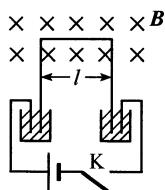
\includegraphics[width=0.2\linewidth]{figures/fig_6_4.jpg}
\end{center}

\vfill

\newpage

\textbf{6.5.} 如习题 6.5 图所示, 斜面上放有一木制圆柱, 圆柱质量 m 为 0.25kg, 半径为 R, 长 l 为 10cm. 圆柱上绕有 10 匝导线, 导线回路平面与斜面平行且通过圆柱轴. 设斜面倾角为 $\theta$ , 一均匀磁场竖直向上, 磁感应强度 B 为 0.50T. 问通过回路的电流 I 至少有多大, 圆柱体才不至沿斜面向下滚动?

\begin{center}
    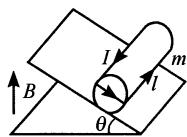
\includegraphics[width=0.2\linewidth]{figures/fig_6_6_1.jpg}
\end{center}
\vfill

\textbf{6.6.} 如习题 6.6 图所示, 一平面塑料圆盘, 半径为 R, 表面带有面密度为 $\sigma$ 的电荷. 假定圆盘绕其轴线 $AA'$ 以角速度 $\omega$ 转动, 磁场 B 的方向垂直于转轴 $AA'$ . 试证磁场作用于圆盘的力矩大小为 $L = \pi \sigma \omega R^{4} B / 4$ .

\begin{center}
    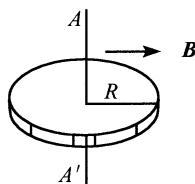
\includegraphics[width=0.3\linewidth]{figures/fig_6_6_2.jpg}
\end{center}

\vfill\newpage

\textbf{6.7} 电流 $I$ 沿半径 $a$ 的导体圆柱壳均匀分布, 通过圆柱轴将导体壳劈成两半, 求两部分单位长度的吸力.



\vfill



\textbf{6.8.} 顺磁质分子的磁矩和玻尔磁矩 $m_{\mathrm{B}} = eh / (4\pi m_{\mathrm{e}})$ 同量级. 设顺磁质温度为 $T = 300\mathrm{K}$ ，磁感应强度 $B = 1\mathrm{T}$ ，问 $kT$ 是 $m_{\mathrm{B}}B$ 的多少倍？ $(h = 6.626\times 10^{-34}\mathrm{J}\cdot \mathrm{s}^{-1}, e = 1.602\times 10^{-19}\mathrm{C}, m_{\mathrm{e}} = 9.11\times 10^{-31}\mathrm{kg}, k = 1.38\times 10^{-23}\mathrm{J}\cdot \mathrm{K}^{-1})$ .

\vfill\newpage

\textbf{6.9.} 一无限长的直圆柱形铜导线外包一层磁导率为 $\mu$ 的圆筒形磁介质，导线半径为 $R_{1}$ ，磁介质的外半径为 $R_{2}$ ，导线内有均匀分布的电流 $I$ 通过。

（1）求导线内、介质内、介质外的磁场强度和磁感应强度的分布。

（2）求介质内、外表面的磁化面电流密度。

\vfill



\textbf{6.10.} 一抗磁质小球的质量为 $0.10\mathrm{g}$ , 密度 $\rho = 9.8\mathrm{g} \cdot \mathrm{cm}^{-3}$ , 磁化率为 $\chi_{m} = -1.82 \times 10^{-4}$ , 放在一个半径 $R = 10\mathrm{cm}$ 的圆线圈的轴线上且距圆心为 $l = 10\mathrm{cm}$ 处 (见习题6.10图). 线圈中载有电流 $I = 100\mathrm{A}$ . 求电流作用在这小球上力的大小和方向.
\begin{center}
    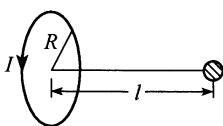
\includegraphics[width=0.3\linewidth]{figures/fig_6_10.jpg}
\end{center}

\vfill\newpage

\textbf{6.11.} 螺绕环的导线内通有电流 20A. 利用冲击电流计测得环内磁感

\vfill



\textbf{6.11.} 环境珠的导线内通有电流 $20\mathrm{A}$ 利用计出电流计测将珠内磁感应强度的大小是 $1.0\mathrm{Wb}\cdot \mathrm{m}^{-2}$ . 已知环的周长是 $40\mathrm{cm}$ , 绕有导线 400 匝. 计算 

(1) 磁场强度; 

(2) 磁化强度; 

(3) 磁化率; 

(4) 磁化面电流和相对磁导率.

\vfill\newpage

\textbf{6.12.} 一半径为 a 的无限长磁介质圆柱, 磁导率为 $\mu$ , 柱外为真空, 沿圆柱轴有一线电流 I, 求磁介质中的磁场强度和磁感应强度以及磁介质圆柱表面的束缚电流分布.

\vfill


\textbf{6.13.} 在空气(相对磁导率 $\mu_{r}=1$ ) 和软铁 ( $\mu_{r}=7000$ ) 的交界面上, 软铁上的磁感应强度 B 与交界面法线的夹角为 $85^{\circ}$ , 求空气中磁感应强度与交界面法线的夹角.
\vfill

\newpage

\textbf{6.14} 如习题 6.14 图所示, 一半无限大磁导率为 $\mu_{1}$ 的磁介质表面放一磁导率为 $\mu_{2}$ 的无限长磁介质半圆柱, 半径为 $a$ . 设在 $A, B$ 两处置入反向直线电流 $I$ , 电流方向与圆柱轴平行. 求空间磁感应强度的分布.

\begin{center}
    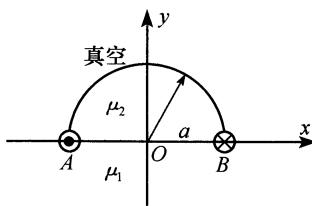
\includegraphics[width=0.3\linewidth]{figures/fig_6_13.jpg}
\end{center}

\vfill

\textbf{6.15} 在一理想导体平面上方的真空中有一圆载流线圈, 线圈平面与导体平面平行, 相距为 $d$ . 设线圈电流为 $I$ , 半径为 $a$ , 求圆线圈轴线上磁感应强度的分布. 当 $a \ll d$ 时, 求圆线圈所受的浮力.

\vfill\newpage

\textbf{6.16} 一无穷长直载流导线和一无穷长磁介质圆柱平行, 导线和圆柱轴的距离为 $d$ , 电流为 $I$ , 介质圆柱半径为 $a$ , 磁导率为 $\mu$ , 求单位长度导线上所受的力.


\vfill

\textbf{6.17.} 已知一个电磁铁由绕有 $N$ 匝载流线圈的 $C$ 形铁片 $(\mu \gg \mu_0)$ 所构成(见习题6.17图). 如果电磁铁的横截面积为 $A$ ，电流为 $I$ ，空隙宽度为 $d, C$ 形铁片各边的长度同为 $l$ ，求空隙中的磁感应强度.

\begin{center}
    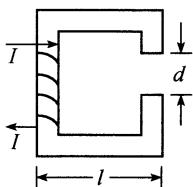
\includegraphics[width=0.2\linewidth]{figures/fig_6_19_1.jpg}
\end{center}

\vfill

\newpage

\textbf{6.18.} 请你设计一块磁铁(使用最少量的铜)，使得在横截面积为 $1\mathrm{m}\times 2\mathrm{m}$ ，长为 $0.1\mathrm{m}$ 的气隙中产生 $10^{4}\mathrm{G}$ 的磁场.假定铁芯的磁导率很高，计算所消耗的功率与所需铜的质量，以及磁铁两磁极之间的引力.(已知铜的电阻率是 $2\times 10^{-6}\Omega \cdot \mathrm{cm}$ ，密度是 $8\mathrm{g}\cdot \mathrm{cm}^{-3}$ ，容许通过的最大电流密度是 $1000\mathrm{A}\cdot \mathrm{cm}^{-2}$ .）

\vfill

\textbf{6.19.} 如习题 6.19 图所示, 设 $L=20cm, L_{g}=0.5cm, \mu_{r}=1200$ , 磁动势 $\varepsilon_{m}=597A$ , 求通过气隙的磁感应强度.

\begin{center}
    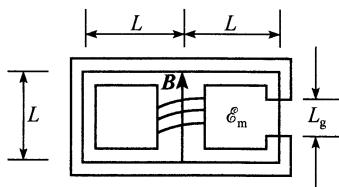
\includegraphics[width=0.3\linewidth]{figures/fig_6_19_2.jpg}
\end{center}

\vfill

\newpage

\textbf{6.20} 一长铁芯沿轴向插入一长螺线管内, 铁芯由两节拼凑而成, 求两节之间的吸力. 设螺线管单位长度匝数为 $n$ , 电流为 $I$ , 铁芯截面积为 $S$ , 磁导率为 $\mu$ .

\vfill

\textbf{6.21} 一圆柱形永磁铁, 直径 $10\mathrm{mm}$ , 长 $100\mathrm{mm}$ , 均匀磁化后磁极化强度 $J = 1.20\mathrm{Wb} \cdot \mathrm{m}^{-2}$ .

(1) 求它两端的磁极强度(即总磁荷量);

(2) 求它的磁矩；

(3) 求磁铁中心处的磁场强度 H 和磁感应强度 B. 此外, H 和 B 的方向有什么关系?

\vfill

\newpage

\textbf{6.22} (1) 一圆磁盘半径为 $R$ , 厚度为 $l$ , 片的两面均匀分布着磁荷, 面密度分别为 $\sigma_{\mathrm{m}}$ 和 $-\sigma_{\mathrm{m}}$ (见习题 6.22 图). 求轴线上离圆心为 $x$ 处的磁场强度 $\pmb{H}$ .

(2) 此磁盘的磁偶极矩 $p_{m}$ 和磁矩 m 为多少?

(3) 试证明, 当 $l \ll R$ 时, 磁盘外轴线上的磁场分布与一个磁矩和半径相同的电流环所产生的磁场一样.



\begin{center}
    \includegraphic